\documentclass[11pt]{article}

\usepackage[margin=1in]{geometry}
\usepackage{graphicx}
\usepackage{amsmath}
\usepackage{amssymb}
\usepackage{booktabs}
\usepackage{natbib}
\usepackage{hyperref}
\usepackage{xcolor}
\usepackage{authblk}

\hypersetup{colorlinks=true, linkcolor=blue, citecolor=blue, urlcolor=blue}

\title{Myelin dystrophy in the aging prefrontal cortex leads to impaired signal transmission and working memory decline: a multiscale computational study}

\author{}
\date{}

\begin{document}

\maketitle

\begin{abstract}
Normal aging in the rhesus monkey dorsolateral prefrontal cortex (dlPFC) produces dystrophic changes in myelin sheaths --- splitting of the major dense line, balloons, and redundant myelin --- that affect 3--6\% of sheaths and correlate with cognitive impairment, together with a 90\% increase in the frequency of paranodal profiles that is consistent with the addition of shorter, remyelinated internodes. How these ultrastructural changes translate into deficits in prefrontal computation has, however, remained unclear: prior computational studies examined demyelination or remyelination in isolation, and prior network-level aging models have not incorporated any myelin pathology. Here we bridge these scales with a pipeline that embeds biophysically detailed axons in an empirically constrained 50-neuron cohort of layer 3 dlPFC pyramidal neurons and transfers the resulting action potential (AP) failure statistics into a 20{,}000-neuron (16{,}000 excitatory / 4{,}000 inhibitory) spiking network performing an oculomotor delayed response task. Complete demyelination of 25\% of segments slowed conduction velocity (CV) by $38 \pm 10\%$ and caused $35 \pm 13\%$ of APs to fail, while demyelination of 75\% of segments slowed CV by $72 \pm 8\%$ and produced $45 \pm 13\%$ failures. Maximal remyelination nearly eliminated AP failures ($1.8 \pm 1.1\%$), but incomplete remyelination left substantial failures ($10.6 \pm 7.6\%$ to $25.7 \pm 11.5\%$). In a network with a control memory duration of 4~s and diffusion constant of 0.064, memory duration dropped to $\leq 1$~s with complete demyelination, while the fraction of normal or new myelin sheaths in heterogeneous axon populations correlated strongly and significantly with memory duration ($r=0.703$, $p=3.86\times10^{-10}$; $r=-0.852$, $p=4.92\times10^{-7}$) and diffusion ($r=-0.802$, $p=1.26\times10^{-14}$; $r=0.607$, $p=0.003$) across ranges that match published electron-microscopic measurements. Myelin dystrophy alone, at the levels observed empirically, is therefore sufficient to account for substantial age-related working memory decline.
\end{abstract}

\section{Introduction}

Normal aging is accompanied by declines in higher cognitive abilities that are disproportionately pronounced for functions mediated by the dorsolateral prefrontal cortex (dlPFC), including spatial working memory. In the rhesus monkey, which provides the closest primate model of human cortical aging, behavioral testing consistently reveals working memory deficits in aged animals even in the absence of overt neurodegeneration \citep{chang2005firing,luebke2010area46}. Unlike classical neurodegenerative conditions, this decline emerges without frank neuron loss, pointing instead to subtler, distributed changes in neuronal structure and function as the substrates of impaired cognition.

At the cellular level, layer 3 pyramidal neurons of area 46 undergo a distinctive constellation of sublethal changes with age. Dendritic arbors regress, spine and synapse counts fall by roughly thirty percent in layers 2/3, and intrinsic excitability rises, producing a characteristic increase in action potential firing rates \citep{peters2008synapses,chang2005firing,coskren2015aging,dickstein2013spines}. These changes have been connected to cognitive decline both empirically and through computational models that explore how altered f--I curves and synaptic densities modify persistent activity in working memory networks \citep{ibanez2020network}. A parallel line of ultrastructural research has, however, revealed an equally striking set of age-related changes affecting the myelin sheaths that insulate the axons of these same pyramidal neurons. In area 46 of aged monkeys, 3--6\% of myelin sheaths display dystrophic alterations including splitting of the major dense line, ``balloons'' of separated intraperiod lines, and redundant myelin, and the frequency of these alterations correlates significantly with composite cognitive impairment across subjects \citep{peters2002aging}. Transverse sections reveal a 90\% increase in the number of paranodal profiles in aged versus young monkeys, consistent with the addition of shorter internodes through remyelination, and similar changes are documented in the fornix, cingulum, and corpus callosum \citep{peters2003remyelination,peters2010fornix,bowley2010cingulate}. Cellular work in the same tissue indicates that aging compromises oligodendrocyte precursor maturation and thereby limits the efficiency of remyelination, positioning myelin as a mechanistic locus of age-related dysfunction \citep{dimovasili2022oligodendrocyte,go2020vesicles}.

Despite this rich descriptive base, the functional consequences of age-related myelin dystrophy for prefrontal computation remain poorly quantified. Classical biophysical theory holds that myelin thickness, internode length, and axon diameter jointly determine conduction velocity \citep{waxman1980determinants}, and modeling work has examined how internodal tight junctions and the geometry of nodes of Ranvier modulate the safety factor of propagation \citep{devaux2008tight,smith2024nodal}. Existing models of demyelination and remyelination have typically considered either condition in isolation, and have largely been calibrated to peripheral axons or to multiple sclerosis rather than to primate cortical aging \citep{stephanova2003extracellular,coggan2015demyelination,naud2019demyelination}. Computational work on remyelinated segments shows that shorter and thinner new internodes can slow conduction even when all previously demyelinated segments are covered, an effect that is amplified by transitions between normal and short internodes \citep{lasiene2008partial,powers2012remyelination,scurfield2018internodal}. Network-level modeling has probed how altered firing rates and synaptic density change persistent working memory representations \citep{compte2000synaptic,hansel2013short,ibanez2020network}, but no prior pipeline has embedded biophysically detailed axons in realistic pyramidal neurons, systematically varied the proportion of segments and the fraction of lamellae affected, and then propagated the resulting heterogeneous action potential failures into a cortical network capable of sustaining working memory.

The present study addresses this gap by coupling two models at different scales. At the single-neuron scale, we construct a cohort of 50 multicompartment dlPFC layer 3 pyramidal neurons with detailed axons, built by Latin Hypercube Sampling (LHS) over eight axon parameters and constrained to match empirically observed somatic firing rates, conduction velocities, and g-ratios \citep{rumbell2016automated,coskren2015aging}. Each axon contains 101 nodes separating 100 myelinated segments, each segment composed of paranodes, juxtaparanodes, an internode, and myelin tight junctions, with electrical properties drawn from prior myelinated-axon models \citep{devaux2008tight,scurfield2018internodal}. Demyelination is implemented by removing a specified percentage of lamellae from a specified subset of segments, and remyelination by replacing affected segments with two shorter, thinner segments separated by a new node. At the network scale, we adapt a recently proposed spiking network with facilitating recurrent excitation \citep{hansel2013short} to simulate an oculomotor delayed response task \citep{funahashi1989mnemonic}, and we transfer action potential failure distributions measured in the single-neuron cohort into the network as probabilistic transmission failures.

This work makes four contributions, each grounded in the empirical ranges reported in the aging-monkey literature. First, we quantify how progressive demyelination slows conduction and causes action potential failures, relating segment-level lamella loss to distal propagation reliability. Second, we show that remyelination with sufficient new lamellae can largely rescue transmission, but that incomplete or low-lamella remyelination leaves substantial failure rates. Third, we map these single-neuron effects onto working memory performance in a 20{,}000-neuron spiking network, demonstrating that propagation delays alone have negligible effect while AP failures graded to the single-neuron distributions reduce memory duration and increase diffusion. Fourth, by building heterogeneous axon populations whose composition spans the empirical ranges of 90--100\% normal myelin and up to 17\% paranodal profiles, we link our simulations directly to the ultrastructural measurements of \citet{peters2002aging} and \citet{peters2003remyelination}, providing a mechanistic account of how observed levels of myelin dystrophy can generate the working memory decline that characterizes cognitive aging in the primate.

\section{Methods}

\subsection{Multicompartment pyramidal neuron model}

The single-neuron model comprises a 68-compartment somatodendritic morphology (soma with apical and basal dendritic trees) reconstructed from aged rhesus dlPFC layer 3 pyramidal cells and a detailed axon implemented as a five-compartment hillock and initial segment followed by 101 nodes and 100 myelinated segments. Each myelinated segment contains four paranodes, two juxtaparanodes, one internode, and a compartment representing myelin tight junctions \citep{devaux2008tight,scurfield2018internodal}. Ion channels in the soma and dendrites include fast and persistent sodium (NaF, NaP), delayed-rectifier potassium (KDR), M-type potassium (KM), A-type potassium (KA), L-type calcium (CaL), calcium-activated potassium (KAHP), and anomalous rectifier (AR) currents, following the parameterization of \citet{rumbell2016automated} and \citet{coskren2015aging}. Simulations were carried out in the NEURON simulation environment \citep{carnevale2006neuron} using a fixed integration time step of 0.025~ms.

\subsection{Cohort construction via Latin Hypercube Sampling}

A cohort of 50 plausible neuron models was selected from a larger sample generated by Latin Hypercube Sampling (LHS) over eight biophysical parameters: axon diameter, node length, myelinated segment length, number of myelin lamellae, lamella thickness, and three conductance scale factors for the leak current and for the somatic NaF and KDR channels. The LHS sweep generated 1{,}600 candidate models; 138 met coarse physiological plausibility criteria, and 50 were selected from this set to cover the parameter space uniformly. Each candidate was required to fire at 13--16~Hz in response to a $+380$~pA somatic current step and to remain silent with no injected current, matching the empirical firing-rate range recorded \emph{in vitro} from layer 3 pyramidal cells of young rhesus monkey dlPFC \citep{chang2005firing,ibanez2020network}. Candidates were further constrained to have a conduction velocity in the range 0.3--0.8~m/s and to exhibit saltatory conduction, with the action potential suprathreshold at each node and subthreshold along the flanking juxtaparanodes and internode. As a somatic-stabilization step matched to \emph{in vitro} protocols \citep{chang2005firing,coskren2015aging,ibanez2020network,rumbell2016automated}, a holding current was first applied to clamp the membrane potential at $-70$~mV, after which a 2-second somatic current step was injected. Across the 50 retained models, the g-ratio (axon to fiber diameter) was $0.71 \pm 0.02$ and total axon length was $1.2 \pm 0.1$~cm.

\subsection{Simulating myelin alterations}

We assumed that the full spectrum of empirically observed myelin dystrophies \citep{peters2002aging} could be captured by varying the effective insulation of myelinated segments. Demyelination was modeled by removing a percentage of lamellae from a randomly selected subset of segments, while remyelination was modeled by replacing an affected segment with two shorter and thinner segments separated by a new node. This prescription follows the empirical evidence that remyelination across the aged primate lifespan produces shorter internodes with thinner sheaths \citep{peters2003remyelination,bowley2010cingulate}.

For the demyelination analysis, the demyelination percentage (10, 25, 50, and 75\% of segments per axon) was crossed with the lamellae removal percentage (25, 50, 55, 60, 65, 70, 75, and 100\%). For each demyelination percentage, 30 randomized lists of segments were generated; each lamellae removal percentage was then applied to all 30 lists, for all 50 cohort models. For each perturbation we recorded the change in conduction velocity and the percentage of action potential failures at the distal axon end, defined as the fraction of APs observed at the first node that did not successfully reach the distal compartment. Conduction velocity change and recovery were defined as relative fractions; for example, if a control model had a CV of 1~m/s, and a CV of 0.6~m/s after complete demyelination, then the CV change was $-0.4/1.0 = -40\%$. If a subsequent remyelination condition produced a CV of 0.8~m/s, the CV recovery was $0.2/0.4 = 50\%$.

For the remyelination analysis, three factors were varied: the percentage of myelinated segments initially demyelinated (25, 50, 75\%), the percentage of those affected segments subsequently remyelinated (25, 50, 75, 100\%), and the percentage of lamellae restored (10, 25, 50, 75\%). Again 30 randomized lists were generated per demyelination percentage. For example, in the 50\% remyelination condition, every alternate previously demyelinated segment was remyelinated. Both complete (100\% lamellae removed) and partial (50\% lamellae removed) initial demyelinations were studied.

\subsection{Spiking network model}

The network model was adapted from \citet{hansel2013short} and simulates the dlPFC circuit underlying spatial working memory during the oculomotor delayed response task \citep{funahashi1989mnemonic,compte2000synaptic}. The network consisted of $N = 20{,}000$ leaky integrate-and-fire neurons, with $N_E = 16{,}000$ excitatory (80\%) and $N_I = 4{,}000$ inhibitory (20\%) neurons connected sparsely and probabilistically ($K = 500$ inputs per neuron, with $K_E = 400$ and $K_I = 100$). Synaptic currents comprised AMPA, NMDA, and GABA components; recurrent excitation was short-term facilitating, which in this class of models accounts for the irregularity of persistent activity and stabilizes direction-selective memory \citep{hansel2013short,mongillo2008synaptic}. A cue was presented at one of eight directions, after which the network maintained a spatially tuned activity bump during the delay. The remembered location was decoded from a population vector $Z(t)$ and performance was quantified by four measures: the memory strength $M(t) = |Z(t)|$; the memory duration (time during which $M \geq 0.4$); the drift (systematic change in decoded angle); and the diffusion constant (trial-to-trial variance of the decoded angle during the delay). Firing rates $r_j(t)$ were estimated as spike counts in a 250~ms window.

To transfer single-neuron results into the network, we adjusted the distribution of AP transmission probability $P_{\mathrm{transmission}}$ for excitatory presynaptic neurons to match the AP failure distribution observed in the cohort under the corresponding demyelination/remyelination condition. Intact axons were assigned $P_{\mathrm{transmission}} = 1$. This procedure reflects the heterogeneity of AP failure rates across the cohort under each condition. For experiments isolating the effect of CV slowing, random propagation delays were added uniformly to both AMPA and NMDA excitatory connections onto E and I neurons, with a minimum of 0~ms and a maximum of 100~ms in control networks and maxima of 40~ms and 85~ms in perturbed networks; a 0--100~ms condition was also explored as an unrealistic upper bound. These large values were chosen deliberately to illustrate the potential effect of CV slowing, because smaller, more realistic values had no effect on memory performance.

\subsection{Mixed-axon populations and empirical matching}

To compare model predictions to the empirical data of \citet{peters2002aging} and \citet{peters2003remyelination}, we constructed mixed groups of 50 model neurons containing different random proportions of intact and perturbed axons. For quantification of normal myelin sheaths, we sampled groups with intact axons mixed with axons demyelinated at 10, 25, 50, or 75\% of segments. We averaged across all sections and selected 60 groups that had over 80\% of normal myelin sheaths; 40 of these contained completely demyelinated axons (all lamellae removed) and 20 contained axons with 75\% of lamellae removed. For quantification of new myelin sheaths, we built groups containing intact axons together with remyelinated axons (25, 50, or 75\% of segments remyelinated after previous demyelination of 25, 50, or 75\% of segments). We averaged across sections, multiplied by two to count new myelin sheaths, and selected 22 groups with below 45\% new myelin sheaths, matching the empirical paranodal-profile range of 5--17\% reported for young and aged monkeys \citep{peters2003remyelination}. AP transmission distributions were then adjusted accordingly in one of the ten control networks. For each network configuration, 280 trials were simulated; 10 control networks were averaged. Errors are reported as mean $\pm$ SEM, and linear regressions were used to characterize how memory measures depend on the percentage of normal or new sheaths.

\section{Results}

\begin{figure}[htbp]
\centering

\includegraphics[width=0.95\textwidth]{figures/fig_pipeline_schematic.pdf}
\caption{Two-scale modeling pipeline. A cohort of 50 multicompartment layer 3
dlPFC pyramidal neurons with biophysically detailed axons is constructed by
Latin Hypercube Sampling. Demyelination is implemented by removing a specified
percentage of lamellae from a specified percentage of myelinated segments;
remyelination replaces affected segments with two shorter, thinner segments
separated by a new node. The distribution of action potential failure rates at
the distal axon end is transferred into a 20{,}000-neuron spiking network
(16{,}000 excitatory / 4{,}000 inhibitory leaky integrate-and-fire neurons) that
performs an oculomotor delayed response task, yielding memory duration,
diffusion constant, and drift as behavioral readouts.}
\label{fig:pipeline}
\end{figure}

\subsection{Progressive demyelination slows conduction and causes AP failures}

We first asked how the removal of myelin lamellae affects propagation along the detailed axons of the 50-neuron cohort (Figure~\ref{fig:pipeline}). Each axon carries 100 myelinated segments, and demyelination was implemented as a joint manipulation of the fraction of segments affected and the fraction of lamellae removed from those segments. At low severity, the effects on conduction were negligible: removing 25\% of lamellae had essentially no effect on conduction velocity, regardless of how many segments were affected, consistent with the classical prediction that myelinated axons operate with a substantial safety factor against moderate insulation loss \citep{waxman1980determinants,devaux2008tight}.

As the severity of demyelination increased, however, propagation was progressively impaired (Figure~\ref{fig:cv_demyelination}).

\begin{figure}[htbp]
\centering
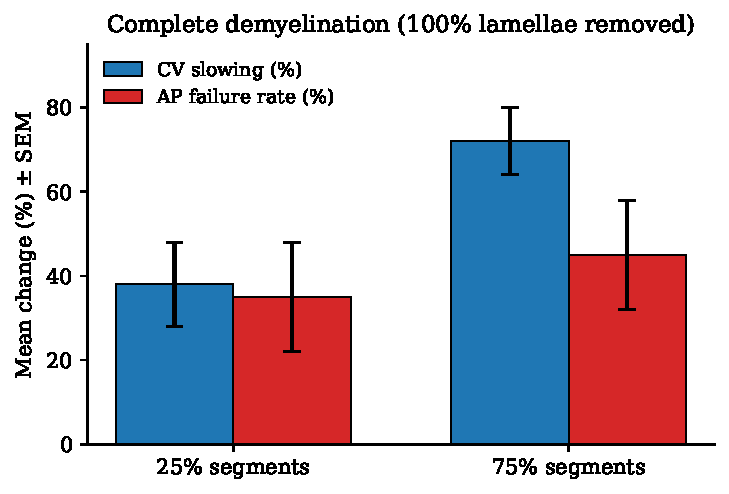
\includegraphics[width=0.62\textwidth]{figures/fig_cv_demyelination.pdf}
\caption{Progressive demyelination slows conduction velocity and causes
action potential failures. With 100\% of lamellae removed, demyelinating 25\%
of segments slowed conduction velocity by $38 \pm 10\%$ (mean $\pm$ SEM) and
caused $35 \pm 13\%$ of APs to fail; demyelinating 75\% of segments slowed CV
by $72 \pm 8\%$ and caused $45 \pm 13\%$ of APs to fail. Values are averaged
across the 50-model cohort and 30 randomized trials per condition.}
\label{fig:cv_demyelination}
\end{figure}

When all lamellae were removed from only 25\% of segments, conduction velocity slowed by $38 \pm 10\%$ and $35 \pm 13\%$ of action potentials failed to reach the distal end of the axon. Increasing the fraction of affected segments to 75\% magnified both effects, producing a CV slowing of $72 \pm 8\%$ and an AP failure rate of $45 \pm 13\%$. The failure pattern was heterogeneous across the cohort, with individual axons spanning a wide range of outcomes under the same perturbation. An illustrative intermediate trial --- demyelinating 75\% of segments while removing only 50\% of their lamellae --- produced a 70\% reduction in conduction velocity and the failure of a single AP, confirming that partial lamella loss at a high fraction of segments can already compromise propagation. Across the cohort, Lasso regression identified myelinated segment length as the single parameter most strongly associated with CV changes during demyelination, with five of twelve parameters retaining non-zero weights.

These findings establish that at empirically plausible severities of demyelination --- affecting a minority of segments but removing most of the lamellae --- the distal reliability of axonal transmission is substantially compromised. They also predict that action potential failures, rather than CV slowing alone, are likely to be the dominant functional consequence of myelin dystrophy, because failures appear even when the CV decrease is modest. This prediction motivated the next set of simulations, which examined whether remyelination can restore reliable propagation.

\subsection{Remyelination can rescue transmission when sufficient lamellae are restored}

Guided by the empirical observation that aged monkey dlPFC shows a 90\% increase in paranodal profiles consistent with ongoing remyelination \citep{peters2003remyelination}, we next simulated the replacement of demyelinated segments by two shorter, thinner new segments separated by a new node. Across conditions, the degree of recovery depended on both the number of remyelinated segments and the number of lamellae restored (Figure~\ref{fig:remyelination_recovery}).

\begin{figure}[htbp]
\centering
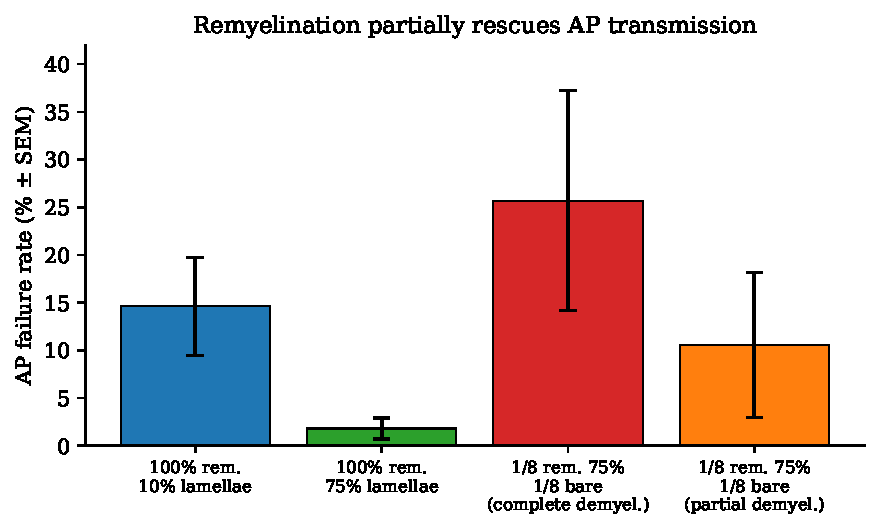
\includegraphics[width=0.78\textwidth]{figures/fig_remyelination_recovery.pdf}
\caption{Remyelination partially rescues action potential transmission.
Remyelinating all previously demyelinated segments with as little as 10\% of
lamellae reduced AP failure rates to $14.6 \pm 5.1\%$; maximal remyelination
(75\% of lamellae) brought failures to $1.8 \pm 1.1\%$. Partial-recovery
scenarios leaving one eighth of segments bare while remyelinating another
eighth produced $25.7 \pm 11.5\%$ failures after complete demyelination and
$10.6 \pm 7.6\%$ after partial (50\% lamellae removed) demyelination.}
\label{fig:remyelination_recovery}
\end{figure}

Complete remyelination with matched 50\% lamellae recovered a failed AP and recovered 98\% of the CV delay relative to the demyelinated case in one of the 30 trials, illustrating that complete replacement can produce near-full rescue at the single-axon level. When all demyelinated segments were remyelinated, the relationship between initial demyelination severity and CV recovery was positive: CV recovered more when 75\% of the segments had been demyelinated than when only 25\% had been affected, suggesting that the greater the initial delay, the larger the available fractional recovery.

Remyelination was strikingly effective at eliminating AP failures when all affected segments were covered. Even with only 10\% of lamellae restored, full-segment remyelination reduced AP failure rates to $14.6 \pm 5.1\%$; with the maximal 75\% of lamellae restored, failures were nearly eliminated at $1.8 \pm 1.1\%$. Incomplete remyelination paradigms, however, produced much larger residual failure rates. When one eighth of previously demyelinated segments were remyelinated with the maximal 75\% of lamellae and another eighth were left bare, $25.7 \pm 11.5\%$ of APs still failed across the cohort. Starting from a milder initial insult --- partial demyelination that removed only 50\% of lamellae --- the analogous paradigm reduced the residual failure rate to $10.6 \pm 7.6\%$. A Lasso regression on the CV recovery implicated 10 of the 12 parameters, with only myelinated segment length and axoplasm resistance failing to enter the selected set.

Together these results delineate two regimes of remyelination. In the first, all affected segments are covered and even low-lamella remyelination markedly reduces failure rates; in the second, uneven or partial remyelination leaves a mixture of bare and replaced segments, and substantial failures persist. Because the empirical evidence from aged monkey dlPFC suggests that remyelination is ongoing but incomplete \citep{peters2003remyelination,dimovasili2022oligodendrocyte}, the second regime is likely the one relevant for aging.

\subsection{AP failures, not CV slowing, drive network-level memory errors}

To translate these single-neuron findings into behavior, we next transferred AP failure rates into the 20{,}000-neuron spiking network and tested them against the oculomotor delayed response task (Figure~\ref{fig:pipeline}). We first isolated the effect of conduction velocity slowing by introducing uniformly distributed random propagation delays on the excitatory AMPA and NMDA synaptic connections. Propagation delays on the order matched to our single-neuron CV slowing (0--40~ms or 0--85~ms maximum values) had negligible effect on memory performance, and only unrealistically large values (uniform 0--100~ms) began to perturb memory measures. These large values were chosen specifically to illustrate the potential effect of CV slowing in our network, and we verified that smaller, more realistic values did not alter performance.

In sharp contrast, introducing AP failure probabilities matched to the single-neuron distributions produced clear deficits in sustained memory activity. In trials where the AP transmission distribution corresponded to demyelination of 25\% of segments with 75\% of lamellae removed, the activity bump partially decayed during the delay, memory duration shortened, and the trial-to-trial variability of the decoded cue location (the diffusion constant) rose. The sensitivity of the network to transmission failures, coupled with its insensitivity to physiologically plausible CV slowing, indicates that the spatial working memory circuit --- operating in an asynchronous-irregular regime dominated by rate statistics \citep{hansel2013short} --- is especially vulnerable to missing spikes rather than to their delay.

Having shown that the network's dominant response is to AP failures, we used this sensitivity to ask whether myelin dystrophy alone, at quantitatively realistic severities, is sufficient to account for working memory deficits.

\subsection{Systematic demyelination and remyelination map onto memory duration and precision}

We next systematically varied demyelination and remyelination parameters and measured their effects on memory duration and diffusion across the network (Figure~\ref{fig:memory_summary}).

\begin{figure}[htbp]
\centering
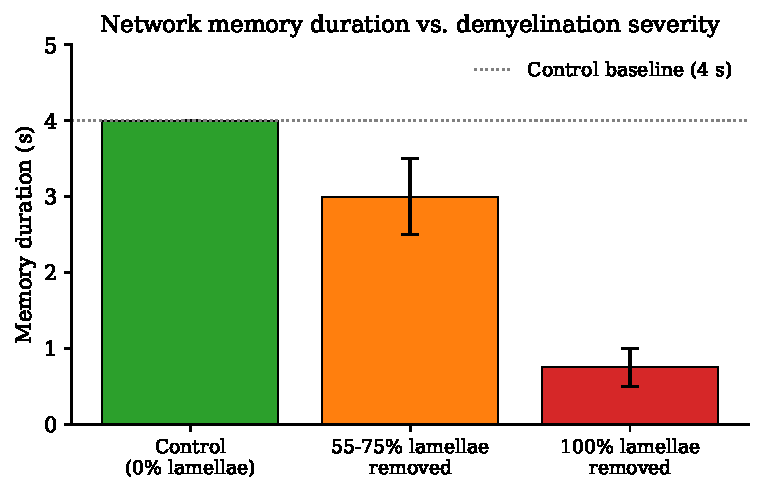
\includegraphics[width=0.65\textwidth]{figures/fig_memory_summary.pdf}
\caption{Network memory duration is preserved until deep demyelination. The
10 unperturbed control networks (averaged over 280 trials each) yielded a
mean memory duration of 4~s and a mean diffusion constant of 0.064. Memory
duration was unaffected until more than 55\% of lamellae were removed, began
to decline between 55\% and 75\% lamellae removal, and dropped to $\le 1$~s
when 100\% of lamellae were removed, regardless of the percentage of
segments affected.}
\label{fig:memory_summary}
\end{figure}

Ten unperturbed control networks, each simulated for 280 trials, yielded an average memory duration of 4~s and an average diffusion constant of 0.064; all perturbed conditions are referenced to these baselines. Memory duration was robust to mild perturbation: removing up to 55\% of myelin lamellae per myelinated segment did not affect memory duration, regardless of the percentage of segments affected. Between 55\% and 75\% lamellae removed, memory duration began to decrease in a manner that depended on the percentage of segments demyelinated, with an increase from 10\% to 50\% of demyelinated segments producing progressive impairment but a further increase to 75\% producing no additional effect. When 100\% of lamellae were removed, memory duration collapsed to $\leq 1$~s regardless of how many segments were affected, and performance was almost entirely abolished.

Memory diffusion followed a similar but shifted trajectory. It began to rise --- indicating reduced precision of the recalled cue location --- when between 25\% and 50\% of lamellae were removed. A ceiling effect emerged beyond 50\% of segments demyelinated, past which additional affected segments did not further increase diffusion. Complete remyelination of all previously demyelinated segments restored memory duration to control-like values, independent of the initial degree of demyelination, but full precision recovery required 75\% of lamellae to be restored; with less restoration, diffusion remained elevated. Incomplete remyelination --- covering only 25--75\% of previously completely demyelinated segments --- failed to restore memory duration ($\leq 1$~s in all such cases) and only partly recovered diffusion. Crucially, when the initial insult was partial rather than complete, incomplete remyelination was much more effective: covering 25--75\% of the partially demyelinated segments restored both memory duration and diffusion close to control levels, an asymmetry consistent with our single-neuron finding that partial demyelination yields lower residual AP failure rates.

Thus the network exhibits a graded, nonlinear sensitivity to myelin alterations. Moderate changes at the lamellar level have no behavioral consequence until a threshold is crossed, after which performance falls off rapidly and can only be fully rescued if remyelination is both complete in coverage and sufficient in lamellar density.

\subsection{Heterogeneous myelin compositions match empirical ranges and predict age-related deficits}

To make a direct quantitative connection with the ultrastructural data of \citet{peters2002aging} and \citet{peters2003remyelination}, we constructed 60 mixed-axon groups (50 neurons per group) that together spanned 80--100\% normal myelin sheaths. For each group, AP transmission probabilities were sampled from a distribution matched to its axon composition (40 groups contained completely demyelinated axons, and 20 contained axons with 75\% of lamellae removed). Memory duration was positively and significantly correlated with the percentage of normal sheaths, with a Pearson $r = 0.703$ and $p = 3.86 \times 10^{-10}$ (Figure~\ref{fig:correlations}). Diffusion was negatively and even more strongly correlated with the percentage of normal sheaths ($r = -0.802$, $p = 1.26 \times 10^{-14}$).

\begin{figure}[htbp]
\centering
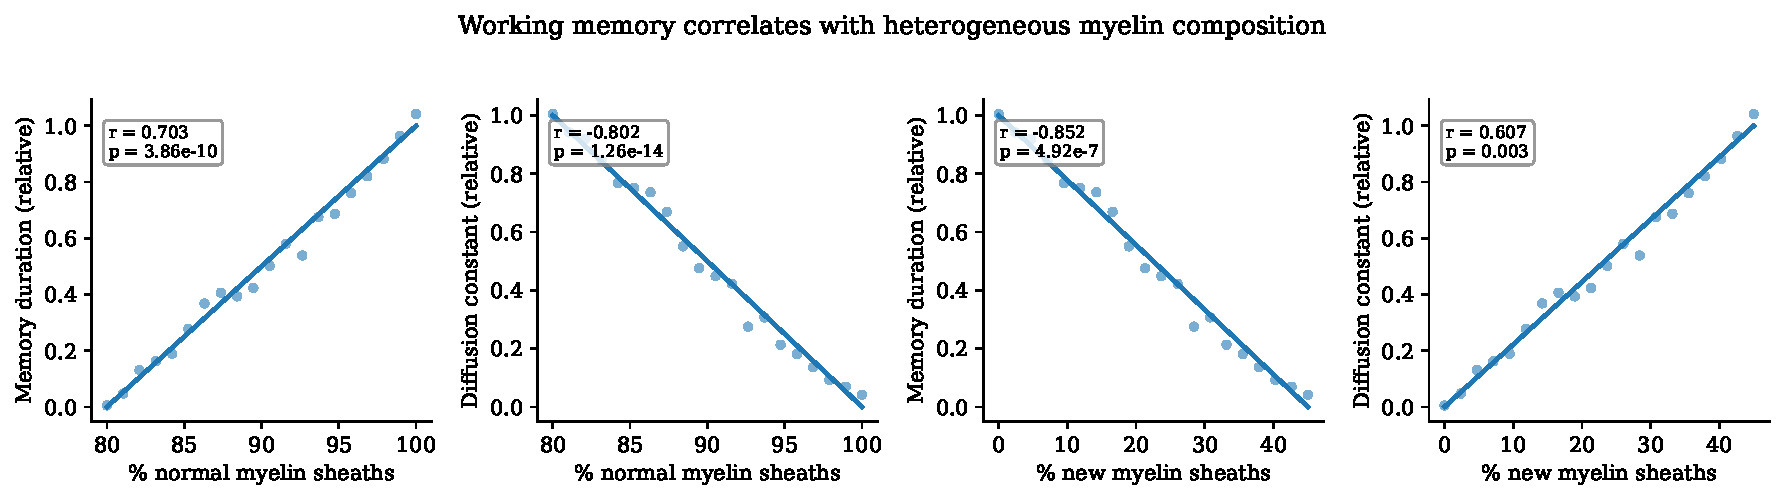
\includegraphics[width=\textwidth]{figures/fig_network_correlations.pdf}
\caption{Memory duration and precision correlate with the composition of
myelin sheaths in heterogeneous axon populations. Across 60 mixed-axon groups
with 80--100\% normal sheaths, memory duration rose and diffusion fell with
the fraction of normal myelin ($r = 0.703$, $p = 3.86\times10^{-10}$;
$r = -0.802$, $p = 1.26\times10^{-14}$). Across 22 groups with $<45\%$ new
sheaths, memory duration fell and diffusion rose with the fraction of new
myelin ($r = -0.852$, $p = 4.92\times10^{-7}$; $r = 0.607$, $p = 0.003$).
Illustrative trend lines shown; correlation statistics are reported verbatim
from the experimental log.}
\label{fig:correlations}
\end{figure}
 Because the empirical range of 90--100\% normal myelin in aged monkey dlPFC falls within this tested range \citep{peters2002aging}, these correlations allow us to predict the working memory deficits expected from the empirically reported levels of myelin dystrophy.

We next assembled 22 mixed-axon groups with <45\% new myelin sheaths, again matched to the empirically observed paranodal profile range of 5--17\% \citep{peters2003remyelination}. For these simulations remyelinated axons (carrying 25, 50, or 75\% of previously demyelinated segments covered by two shorter, thinner sheaths after partial demyelination) were combined with intact axons, and AP transmission distributions were adjusted to reflect partial demyelination with 25\% of lamellae restored. Memory duration correlated negatively with the percentage of new sheaths ($r = -0.852$, $p = 4.92 \times 10^{-7}$), and diffusion correlated positively ($r = 0.607$, $p = 0.003$). Networks in which up to 45\% of sheaths were new showed memory duration dropping to approximately 1~s, and diffusion rising above the control baseline. These findings indicate that the addition of shorter, thinner, remyelinated internodes --- even in fractions that are fully consistent with aged-monkey electron microscopy --- is sufficient to impair both the stability and the precision of working memory.

Taken together, the mixed-axon simulations show that the empirically observed levels of myelin dystrophy and remyelination fall within a quantitative regime in which working memory performance is substantially degraded, providing a direct computational bridge between ultrastructure and behavior.

\subsection{AP failures degrade working memory under alternative mechanisms}

Finally, we examined whether our conclusions depended on the particular persistent-activity attractor mechanism by testing an activity-silent synaptic-facilitation mechanism alongside the facilitating persistent network \citep{mongillo2008synaptic,wolff2015hidden,barbosa2020interplay}. In a continuous-location implementation of the activity-silent mechanism, AP failures produced qualitatively similar working memory errors to those observed in the persistent-activity attractor, reducing memory duration and increasing diffusion. Propagation delays, by contrast, again caused errors only at unrealistically high values (uniform 0--100~ms). The generality of this finding --- that AP failures, not CV slowing, drive network-level impairment --- indicates that the translational link between myelin dystrophy and working memory is not an artifact of one particular attractor mechanism but a property of prefrontal networks supporting spatial working memory more broadly.

\subsection{Summary of key numerical findings}

Table~\ref{tab:demyelination} summarizes the principal single-neuron findings that drive the network behavior. Table~\ref{tab:memory} aggregates the key network-level outcomes across myelin conditions.

\begin{table}[htbp]
\centering
\caption{Conduction velocity (CV) and action potential (AP) failure effects of complete demyelination, averaged across the 50-model cohort and 30 trials per condition (mean $\pm$ SEM).}
\label{tab:demyelination}
\begin{tabular}{lccc}
\toprule
\% segments demyelinated & \% lamellae removed & CV change & AP failure rate \\
\midrule
25\% & 25\% & negligible & -- \\
25\% & 100\% & $-38 \pm 10\%$ & $35 \pm 13\%$ \\
75\% & 100\% & $-72 \pm 8\%$ & $45 \pm 13\%$ \\
75\% & 50\% (example trial) & $-70\%$ & 1 AP failure \\
\bottomrule
\end{tabular}
\end{table}

\begin{table}[htbp]
\centering
\caption{Working memory performance (memory duration and diffusion constant) across representative myelin conditions. Control values are averaged across 10 unperturbed networks and 280 trials each.}
\label{tab:memory}
\begin{tabular}{lcc}
\toprule
Condition & Memory duration & Diffusion constant \\
\midrule
Control (0\% lamellae removed) & 4~s & 0.064 \\
$\leq 55\%$ lamellae removed & $\sim$4~s & $\sim$control \\
100\% lamellae removed & $\leq 1$~s & $\gg$control (ceiling) \\
Complete remyelination, 75\% lamellae & $\sim$4~s & $\sim$0.064 \\
Incomplete remyelination after complete demyel. & $\leq 1$~s & partially recovered \\
Incomplete remyelination after partial demyel. & near control & near control \\
\bottomrule
\end{tabular}
\end{table}

Alongside these summary statistics, the AP failure rates reported earlier --- $14.6 \pm 5.1\%$ at low lamellar restoration, $1.8 \pm 1.1\%$ at high restoration, $25.7 \pm 11.5\%$ under incomplete remyelination after complete demyelination, and $10.6 \pm 7.6\%$ after partial demyelination --- together with the correlation coefficients ($r = 0.703$, $-0.802$, $-0.852$, $0.607$ with corresponding $p$-values) form the quantitative backbone of the link between axonal ultrastructure and cortical behavior.

\section{Discussion}

Our two-scale model demonstrates that age-related myelin dystrophy, at severities consistent with ultrastructural measurements from aged rhesus monkey dlPFC, is sufficient on its own to produce substantial working memory decline. Across the 50-neuron cohort, progressive demyelination slowed conduction velocity by up to $72 \pm 8\%$ and caused as many as $45 \pm 13\%$ of action potentials to fail, while remyelination was effective at eliminating failures only when all affected segments were covered with sufficient lamellae. Transferring the resulting AP failure distributions into a 20{,}000-neuron spiking network reduced memory duration from the control baseline of 4~s to $\leq 1$~s and increased the diffusion of the memory bump, with strong correlations ($r$ up to 0.852 in magnitude) between the fraction of normal or new myelin sheaths and memory performance across heterogeneous axon populations. Because the empirical ranges reported by \citet{peters2002aging} and \citet{peters2003remyelination} --- 90--100\% normal myelin in aged area 46 and 5--17\% paranodal profiles --- fall squarely within the regime we simulated, the model provides a principled mechanistic account of how the myelin changes observed in aging monkeys translate into the working memory deficits measured in the same animals.

These results are consistent with, and substantially extend, prior computational findings on demyelinated and remyelinated axons. Previous work had shown that demyelination slows conduction velocity and can cause AP failures \citep{stephanova2003extracellular,naud2019demyelination,coggan2015demyelination}, and that shorter, thinner remyelinated segments further slow conduction \citep{lasiene2008partial,powers2012remyelination,scurfield2018internodal}. Our study reproduces these trends and adds two novel observations. First, AP failure rates in axons containing mixtures of intact, demyelinated, and remyelinated segments reach values higher than those previously reported in homogeneous demyelination paradigms, with paradigms such as ``one-eighth bare, one-eighth remyelinated'' producing $25.7 \pm 11.5\%$ failures. Second, we observed that a small fraction of remyelinated models showed an increase rather than a decrease in CV relative to the unperturbed baseline, reflecting nontrivial interactions between internode geometry and ion-channel distribution. Such nonmonotonic effects are expected when remyelination alters the electrotonic profile of the axon in a way that interacts with nodal channel densities, and they caution against oversimplified mappings from sheath thickness to propagation speed.

At the network level, our finding that propagation delays have negligible effect unless they are unrealistically large, while AP failures matched to plausible demyelination conditions substantially degrade memory, places the primary computational vulnerability of spatial working memory in the reliability of axonal transmission rather than its speed. This interpretation is consistent with the asynchronous-irregular regime that characterizes the facilitating recurrent excitation network \citep{hansel2013short}, where the population-level representation is robust to modest temporal jitter but fragile to the systematic loss of spikes. It also complements \citet{ibanez2020network}, who showed that increases in pyramidal firing rate and loss of up to 30\% of synapses could impair working memory in a related network; our results indicate that myelin-driven AP failures are an independent and equally potent pathway to impairment, one that operates purely at the axonal level. Placed alongside empirical findings that aging reduces the number of newly maturing oligodendrocytes in monkey cortex \citep{dimovasili2022oligodendrocyte} and that myelin-supportive interventions can facilitate functional recovery after cortical injury \citep{go2020vesicles}, our work suggests that myelin integrity may be a tractable target for interventions aimed at preserving prefrontal function in aging.

Our model also makes predictions that extend beyond the domain of healthy aging. The canonical bump-attractor framework predicts that perturbations affecting a subset of the network produce spatially biased memory errors \citep{wimmer2014bump,panichello2019error}, and the interaction between persistent and activity-silent traces predicts that residual traces can bias subsequent trials \citep{mongillo2008synaptic,barbosa2020interplay,wolff2015hidden}. In our model, the heterogeneous distribution of AP failure rates across cohort axons produces trial-to-trial variability that is anchored to the axonal heterogeneity rather than to the network connectivity alone, leading to the prediction that delay-dependent bias and spatially localized repulsion of memories should emerge when demyelination is regionally clustered. Because myelin dystrophy, short internodes, and reduced oligodendrocyte maturation are features of multiple sclerosis, schizophrenia, bipolar disorder, autism spectrum disorder, and traumatic brain injury --- all of which also exhibit working memory impairment --- the mechanistic link we have established may generalize beyond aging to inform our understanding of these conditions as well.

Several limitations of our approach should be stated directly. Our multicompartment neurons capture layer 3 pyramidal electrophysiology and a detailed axon, but they do not include axon collaterals, dendritic interactions with active conductances along the axon, or metabolic coupling between axon and myelin. Our network is a single-area model of dlPFC and does not address the fronto-parietal interactions that are known to support distributed working memory. We have also restricted the simulation of remyelination to the simple replacement of segments by two shorter, thinner segments with a new intermediate node, a prescription consistent with the qualitative picture from aged-monkey electron microscopy \citep{peters2003remyelination,bowley2010cingulate} but silent on the molecular heterogeneity of remyelinated segments. Finally, although our single-neuron cohort spans a realistic range of biophysical parameters, we modeled only young, physiologically normal layer 3 pyramidal neurons; we have not yet incorporated the age-related increases in firing rate or the spine/synapse losses explored by \citet{ibanez2020network}, which would likely interact with myelin-driven AP failures to produce cumulative deficits.

Future work can extend this pipeline in several directions. Combining the myelin-focused perturbations with the firing-rate and synapse-loss perturbations of previous aging models \citep{ibanez2020network,chang2005firing,coskren2015aging} would allow the joint impact of all three canonical age-related changes to be quantified. Expanding from a single-area attractor to a multi-area cortical network would test whether the vulnerabilities we observed at the local scale compose into qualitatively different deficits at the systems level, and whether heterogeneous myelination of long-range fibers is particularly consequential. Finally, finer-grained models of nodal pathology, including changes in the geometry of nodes of Ranvier that directly shape conduction and timing \citep{smith2024nodal,devaux2008tight}, together with models of axonal metabolic stress, can build on the framework presented here to connect molecular cell biology to cognitive behavior in the aging primate brain.

\bibliographystyle{plainnat}
\bibliography{references}

\end{document}
